\documentclass[11pt]{article}

\usepackage[a4paper,margin=1in]{geometry}
\usepackage{amsmath}
\usepackage{amssymb}
\usepackage{booktabs}
\usepackage{float}
\usepackage{graphicx}
\usepackage{pdflscape}
\usepackage{tabularx}
\usepackage{tikz}
\usetikzlibrary{arrows.meta,positioning}
\usepackage[hidelinks]{hyperref}
\usepackage[authoryear,round]{natbib}
\usepackage{siunitx}
\sisetup{group-separator={,},group-minimum-digits=4}

\newcommand{\Hnorm}{1-H_{\mathrm{norm}}}

\title{Diagnosing Mitigation Need: Controlled Shortages and\\
Signal-Matched Interventions in Histopathology Patch Classification}
\author{Yannik Queisler}
\date{\today}

\begin{document}
\raggedbottom
\hypersetup{pageanchor=false}
\begin{titlepage}
\centering
\vspace*{\fill}
\makeatletter
{\LARGE\bfseries \@title\par}
\vspace{1.5em}
{\large \@author\par}
\vspace{1.5em}
{\large \@date\par}
\makeatother

\begin{abstract}
\begingroup
\setlength{\emergencystretch}{2em}
\noindent A class can be underserved for several distinct reasons, and the count that marks it as rare does not say which. In computational pathology, raw sample counts hide at least one further shortage --- few labelled patients or slides behind many informative patches --- and say nothing about how separable a class is under the available representation or how much variation it spans. This benchmark uses training allocation as a controlled way to induce such a shortage, and then asks which signal a mitigation method should read to repair it: how would the same prediction task change if one fixed training budget were distributed evenly across classes rather than concentrated in head classes, which signal profile does the resulting condition actually present, and does a method that reads the signal matching that profile recover more of the damage than one that reads a different signal? CAMELYON16, TCGA-UT, BRACS, and PANDA are studied in patch classification using frozen Virchow2 features. Patient- or case-disjoint partitions, natural validation and test cohorts, model family, and optimizer-update budgets remain fixed while only training support is redistributed among size-matched balanced, moderate, and severe conditions. Balanced accuracy and tail-group macro negative log likelihood measure discrimination and probability quality. Mitigation recovery is interpreted only after a prespecified gate establishes a meaningful allocation-induced deficit. A five-member family of methods --- one per signal, all a mean-one class weight on unmodified cross-entropy --- makes the signal contrast interpretable at a fixed intervention level. Exploratory analyses then relate damage and recovery to achieved severity, support--difficulty alignment, and independent support. The benchmark is scoped to patch classification, where each prediction unit carries its own label.
\par
\endgroup
\end{abstract}
\vspace*{\fill}
\end{titlepage}
\hypersetup{pageanchor=true}

\setcounter{tocdepth}{2}
\tableofcontents
\clearpage

\section{Introduction}
Choosing a mitigation method requires first identifying what limits a class. In histopathology patch classification, an underserved class may lack nominal patch support, independent evidence from patients or slides, learnable signal, or representational diversity. These shortages are not interchangeable. Thousands of patches from a few patients may provide less independent evidence than a smaller patch set drawn from many patients, while neither count reveals how difficult a class is to separate or how much variation it contains. A method that responds to one shortage may therefore be ineffective when another shortage limits performance.

This benchmark asks when such a shortage causes enough damage to warrant mitigation and whether recovery improves when a method reads the signal that identifies that shortage. Training allocation provides the controlled intervention needed to answer these questions. For the same task and total training budget, examples are distributed either evenly across classes or concentrated in head classes. A size-matched balanced cross-entropy (CE) model provides the reference. Validation and test cohorts retain their natural class distributions, so the resulting contrast reflects the training allocation rather than a change in the evaluation population.

Allocation is thus a way to create controlled variation in evidence, not the benchmark's main explanatory focus. Each condition is instead characterized by its realized \emph{signal profile}: class prevalence, nominal patch support, independent patient or slide support, class difficulty, and representational diversity. This profile is measured rather than inferred from the nominal imbalance ratio. The companion methods report defines the signal taxonomy and locates each tested method within it \citep{queisler2026imbalanceMethods}; the present benchmark tests whether matching method to signal matters empirically.

The study covers CAMELYON16, TCGA-UT, BRACS, and PANDA using frozen Virchow2 patch features. Patient- or case-disjoint partitions, model family, optimizer-update budget, and natural validation and test cohorts remain fixed while the allocation of a common training budget changes. Balanced, moderate, and severe allocations establish the controlled comparisons. To separate signal choice from intervention mechanism, the confirmatory family contains five methods that all apply a mean-one class weight to unmodified CE. Their weights differ only in whether they use prevalence, nominal support, independent support, difficulty, or diversity.

This design yields three research questions:
\begin{description}
  \item[RQ1.] \textbf{Which shortage does controlled allocation create, and what does it damage?} Under otherwise fixed conditions, how do controlled changes in training allocation affect tail-class discrimination and calibration, and which signal profile does each condition realize?
  \item[RQ2.] \textbf{Does signal-matched mitigation recover more of the damage?} Which methods recover performance lost specifically to training imbalance, and does recovery improve when a method reads the shortage identified in RQ1?
  \item[RQ3.] \textbf{What explains variation in damage and mitigation headroom?} Are achieved imbalance severity and support--difficulty alignment associated with whether damage occurs, how large it is, and how much can be recovered? Separability, learnability, and support measures provide sensitivity analyses.
\end{description}
RQ1 first establishes whether a recoverable deficit exists and which signals characterize it. RQ2 is evaluated only after this deficit passes a prespecified gate. RQ3 then examines why deficit size and recovery headroom vary; it is an exploratory association analysis, not another method ranking.

The benchmark is limited to patch classification because directly labelled patches allow nominal patch support to change within a fixed pool of patients or slides. At whole-slide level, reallocating labelled slides changes nominal and independent support together, making the two signals harder to separate. Dataset provenance and detailed method objectives remain in the companion reports \citep{queisler2026datasets,queisler2026imbalanceMethods}. The next section defines the prediction and evidence units on which the experimental design rests.

\section{Study Setting}
\label{sec:data}
This benchmark covers one prediction regime: patch classification predicts a label for one directly labelled image crop, so every training example carries its own target and the split unit that contains it is the only source of statistical dependence between examples. The terms \emph{patch} and \emph{tile} both denote a $256\times256$ crop, but \emph{patch} is used throughout.

Table~\ref{tab:datasets} defines the prediction example, target, and split unit in each dataset. A \emph{split unit} is the patient or participant where available and the biopsy otherwise. It is assigned to exactly one partition before any imbalance is constructed, and all patches from that unit follow the assignment.

Eligibility is fixed before splitting and construction; Appendix~\ref{app:construction} gives the exclusion and preprocessing rules.

\begin{table}[ht]
  \centering
  \scriptsize
  \begin{tabularx}{\linewidth}{@{}l>{\raggedright\arraybackslash}X>{\raggedright\arraybackslash}X@{}}
    \toprule
    Dataset & Patch-level example and label & Split unit \\
    \midrule
    CAMELYON16 & Non-overlapping tissue crop at \num{20}x; tumor if at least \num{50}\% of its aligned mask cell is tumor, normal otherwise & Slide (one slide per patient) \\
    TCGA-UT & Author-supplied tumor-region crop; inherits its source WSI's cancer type & TCGA participant \\
    BRACS & Non-overlapping crop from a pathologist-annotated ROI; inherits one of seven ROI subtypes & Patient \\
    PANDA & Foreground crop; cancer if at least \num{50}\% of its aligned provider-specific mask cell is cancer, benign otherwise & Biopsy (one WSI) \\
    \bottomrule
  \end{tabularx}
  \caption{Dataset-specific definitions of patch-level examples. TCGA-UT's eligible target set omits one of the 32 annotated cancer types; Appendix~\ref{app:construction} states which class and why.}
  \label{tab:datasets}
\end{table}

Eligible patches are embedded once with frozen Virchow2. Concatenating the CLS token and mean patch token gives 2560 input features \citep{vorontsov2024virchow,zimmermann2024virchow2}. CAMELYON16 and PANDA use mask-derived patch targets, TCGA-UT patches inherit the source WSI's cancer type, and BRACS patches inherit the annotated ROI subtype. The common model is a two-layer multilayer perceptron (MLP); method-specific head changes are listed in Appendix~\ref{app:training}.

With prediction and evidence units fixed, the next question is how to change class allocation without changing the task.

\section{Controlled Experimental Design}
\label{sec:design}
\label{sec:construction}
Training allocation creates controlled differences in the evidence available to each class without changing the task or evaluation population. Four conditions establish the comparison: a full natural anchor, a size-matched balanced reference, a moderate imbalance targeting $\rho=10$, and a severe imbalance targeting $\rho=100$ where feasible. The natural anchor describes performance with all eligible training data and with the dataset's own class prevalence; because it is descriptive, only its CE reference is fitted. Only the three controlled conditions share total support $T$, carry the full method roster, and enter imbalance-deficit and recovery estimands.

\subsection{What changes and what remains fixed}
The design asks a simple counterfactual question: how would the same prediction task perform if a fixed training budget were distributed evenly across classes rather than concentrated in a head class? Within each split, the data source, prediction target, eligible examples, frozen representation, split-unit partition, natural validation and test cohorts, total controlled support, and optimizer-update budget remain fixed. Only class allocation within training support changes. Figure~\ref{fig:controlled-construction} summarizes this separation between fixed choices and the intended intervention.

\begin{figure}[ht]
  \centering
  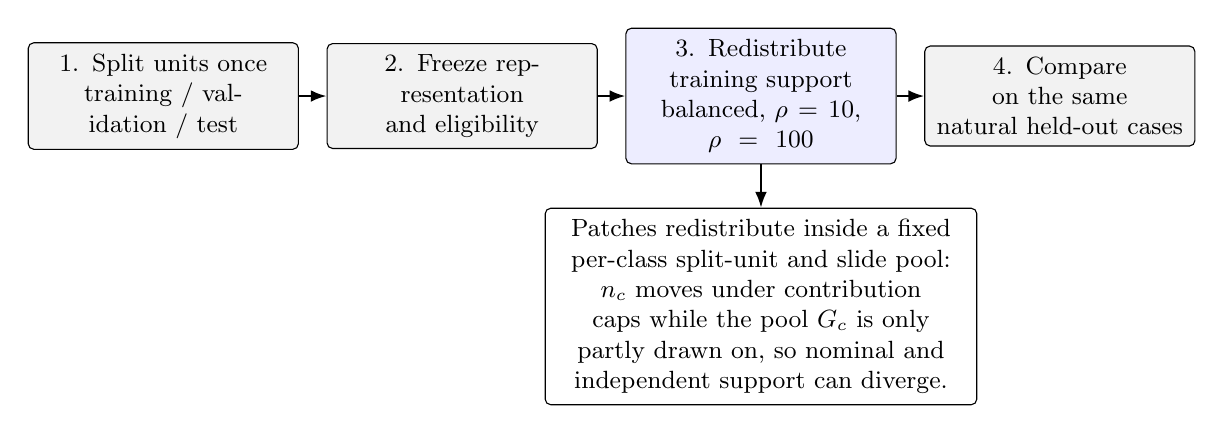
\begin{tikzpicture}[
    box/.style={draw, rounded corners=2pt, align=center, inner sep=4pt, font=\small, text width=3.15cm, minimum height=1.15cm},
    fixed/.style={box, fill=gray!10},
    varied/.style={box, fill=blue!7},
    note/.style={box, fill=white, text width=5.2cm, minimum height=1.0cm},
    arrow/.style={-{Latex[length=2mm]}, thick}
  ]
    \node[fixed] (split) {1. Split units once\\training / validation / test};
    \node[fixed, right=0.35cm of split] (freeze) {2. Freeze representation\\and eligibility};
    \node[varied, right=0.35cm of freeze] (construct) {3. Redistribute training support\\balanced, $\rho=10$, $\rho=100$};
    \node[fixed, right=0.35cm of construct] (evaluate) {4. Compare on the same\\natural held-out cases};
    \node[note, below=0.55cm of construct] (patch) {Patches redistribute inside a fixed per-class split-unit and slide pool: $n_c$ moves under contribution caps while the pool $G_c$ is only partly drawn on, so nominal and independent support can diverge.};
    \draw[arrow] (split) -- (freeze);
    \draw[arrow] (freeze) -- (construct);
    \draw[arrow] (construct) -- (evaluate);
    \draw[arrow] (construct.south) -- (patch.north);
  \end{tikzpicture}
  \caption{Controlled construction of the benchmark. Gray steps are fixed within a split; the blue step is the intended intervention.}
  \label{fig:controlled-construction}
\end{figure}

\noindent The balanced, moderate, and severe conditions contain the same total training support $T$, in patches. The shared $T$ is selected jointly with severity, not from size alone: construction retains the largest feasible total whose realized moderate and severe ratios lie within 10\% of their targets, that is $\rho_{\mathrm{achieved}}\in[9,11]$ and $\rho_{\mathrm{achieved}}\in[90,110]$, for every locked tail assignment. Choosing $T$ from size alone could flatten the intended contrast, and this tolerance keeps both controlled conditions recognizably close to their nominal severities rather than only as separated as the data allow. Appendix~\ref{app:construction} specifies the tolerance search and its feasibility rules.

The target ratio $\rho_{\mathrm{target}}\in\{1,10,100\}$ specifies the intended intervention, but integer allocation and finite inventories can change the realized class distribution. The achieved ratio is therefore recomputed from every realized training set. For realized class supports $N_1,\ldots,N_K$, it is
\begin{equation}
  \rho_{\mathrm{achieved}}=\frac{N_{\max}}{N_{\min}}.
  \label{eq:rho}
\end{equation}
This quantity records the extreme head--tail contrast. The complementary normalized-entropy deficit
\begin{equation}
  \Hnorm=1-\frac{-\sum_{c=1}^{K}p_c\log p_c}{\log K},
  \qquad p_c=\frac{N_c}{\sum_jN_j}.
  \label{eq:entropy}
\end{equation}
\noindent uses all classes and is normalized for class count: it is zero for a balanced allocation and increases as support becomes concentrated. Both quantities are computed from each realized training set. Per-class split-unit, slide, and patch counts are reported alongside them, because neither scalar reveals whether many patches originate from only a few cases.

Split-unit-disjoint training, natural-validation, and natural-test partitions are created first. Imbalance manipulation is confined to training support. Within a split, every condition uses exactly the same validation and test cases and eligible held-out examples. No held-out example is deleted, duplicated, or reweighted according to the training severity. Patch-level evaluation uses every eligible held-out patch. Consequently, recall is estimated from all available held-out cases and prevalence-dependent precision and macro F1 are compared at one fixed test prevalence.

The validation cohort also retains its natural distribution. It is used for hyperparameter and checkpoint selection but never resized to resemble a training condition. Training, validation, and test sample lists are versioned with split-unit identifiers, class counts, construction seed, and content hashes before model fitting.

\subsection{Independent support and feasibility}
\label{sec:independent-support}
\emph{Independent support} $G_c$ is the distinct split units and slides underlying a class, in the sense defined in the companion methods report \citep{queisler2026imbalanceMethods}. Patch conditions draw from a fixed per-class split-unit and slide pool under the contribution caps of Table~\ref{tab:support-rules}, so $G_c\approx\min(|\mathrm{pool}_c|,n_c)$: a severe tail typically tracks its patch count $n_c$, while a head class saturates at its pool size well before $n_c$ does. A preflight check on the frozen training sets, reported alongside the definitive results, confirms this separation is real rather than an artifact of one dataset: across BRACS, CAMELYON16, and PANDA, $G_c$ moves with a class's case pool rather than with $n_c$, sometimes even ranking classes in the opposite order from $n_c$; TCGA-UT is the exception, where most classes' $G_c$ saturates at a common floor regardless of $n_c$. This decoupling is what makes nominal support $n_c$ and independent support $G_c$ distinguishable signals rather than two names for the same quantity (Section~\ref{sec:methods}), and TCGA-UT's near-uniform floor is itself evidence for RQ3 about when independent support stops discriminating between classes at all.

A \emph{support pilot} determines how little independent tail evidence remains defensible before definitive comparisons are built. The definitive floor is the larger of that empirical level and the design floor implied by the contribution caps (Table~\ref{tab:locked}). Conditions that cannot satisfy these floors are weakened or excluded rather than rescued by changing validation or test data.

\subsection{Severity and tail placement}
Severity controls how the shared total $T$ is distributed. Binary tasks have one head and one tail; multiclass tasks place intermediate supports at equal intervals on a logarithmic scale. Requested and achieved ratios are both reported because finite inventories and integer counts can weaken the realized contrast. A condition that collapses to the balanced allocation is recorded as degenerate and never pooled with genuine imbalanced conditions.

Support rank must also be separated from intrinsic class difficulty. Native, difficulty-aligned, and difficulty-reversed \emph{tail assignments} place semantic classes at different points in the same support profile. Aligned assignments compound difficulty with scarcity; reversed assignments compensate difficult classes with greater support. Duplicated assignments are omitted transparently. Appendix~\ref{app:construction} gives contribution caps, pilot quotas, ordering rules, allocation equations, infeasibility handling, and seed families.

\subsection{Prespecified controls}
Every design and training quantity is fixed before the first definitive fit. Table~\ref{tab:locked} collects these controls with a pointer to the specification that derives each one. Deficit gates and resampling rules are introduced later, together with the endpoints they govern.

\begin{table}[H]
  \centering
  \footnotesize
  \begin{tabularx}{\linewidth}{@{}>{\raggedright\arraybackslash}p{0.27\linewidth}Xl@{}}
    \toprule
    Locked quantity & Value & Spec \\
    \midrule
    Representation & Frozen Virchow2 features & \ref{app:construction} \\
    Patch classifier & Two-layer MLP, 512 hidden units & \ref{app:construction} \\
    Update budget & $U=30\lceil T/B\rceil$ optimizer updates & \ref{app:training} \\
    Learning-rate envelope & Seven values, \num{1e-5} to \num{1e-2} & \ref{app:controls} \\
    Support floor per class & $\geq10$ split units and $\geq20$ slides & \ref{app:construction-support} \\
    Contribution caps & $\leq10\%$ per split unit; $\leq5\%$ per slide & \ref{app:construction-support} \\
    Severity targets & $\rho_{\mathrm{target}}\in\{1,10,100\}$ & \ref{app:construction} \\
    Severity tolerance & Achieved $\rho\in[9,11]$ and $[90,110]$ & \ref{app:construction-support} \\
    Tail assignments & Native, difficulty-aligned, difficulty-reversed & \ref{app:construction} \\
    Split-unit partitions & Three locked, patient- or case-disjoint & \ref{app:construction} \\
    Initialization seeds & Two tuning; five disjoint confirmation & \ref{app:training} \\
    \bottomrule
  \end{tabularx}
  \caption{Design and training quantities locked before the first definitive fit, with the section or appendix that specifies each. Only class allocation within the shared training support $T$ varies across controlled conditions.}
  \label{tab:locked}
\end{table}

These safeguards define the evidence available to every model. The next section asks how matched models turn that evidence into damage and recovery estimates.

\section{Measuring Damage and Recovery}
\label{sec:analysis}
RQ1 and RQ2 are answered in a deliberately asymmetric sequence. Balanced CE is compared with imbalanced CE first. Only when that contrast shows a meaningful deficit on discrimination or calibration is a mitigation method interpreted in terms of recovery on the affected endpoint.

For intuition, suppose balanced CE attains balanced accuracy \num{0.72}, imbalanced CE attains \num{0.62}, and a mitigation method attains \num{0.68}. Imbalance caused a \num{0.10} deficit and the method regained \num{0.06}, or 60\% of the demonstrated damage. This normalization distinguishes repair of an imbalance effect from a generic method improvement. Exact estimands and gates appear after the endpoints they use.

\subsection{Methods compared under imbalance}
\label{sec:methods}
Table~\ref{tab:roster} lists only the methods evaluated in this benchmark, grouped by the mitigation signal each one reads rather than by intervention family. This follows the signal--intervention table in the companion methods report so the two remain comparable at a glance. CE is the size-matched no-mitigation reference. The roster is the patch-applicable subset of that report's broader taxonomy; methods that consume a different input form are not evaluated here. The roster is fitted in the balanced, moderate, and severe conditions, which alone supply the paired contrast a mitigation claim requires; the natural anchor carries the CE reference only. Method objectives, tested adaptations, ablations, defaults, and fidelity qualifications are defined exclusively in the companion methods report \citep{queisler2026imbalanceMethods}.

\begin{table}[H]
  \centering
  \scriptsize
  \begin{tabularx}{\linewidth}{@{}>{\raggedright\arraybackslash}p{0.20\linewidth}>{\raggedright\arraybackslash}p{0.30\linewidth}X@{}}
    \toprule
    Signal & Tested methods & Intervention \\
    \midrule
    None (reference) & CE & None \\
    Prevalence & Balanced sampling; weighted CE; train-time and post-hoc logit adjustment; cRT & Sampling; loss weight; logits and prior correction; classifier retraining \\
    Nominal support & Class-balanced CE & Loss weight \\
    Independent support & Independent-support weighted CE & Loss weight \\
    Difficulty & Focal loss; pilot-difficulty weighted CE & Loss weight \\
    Diversity & Semantic-scale weighted CE & Loss weight (dynamic) \\
    Nominal support and difficulty & CFAL & Prototype head and margin loss \\
    Prevalence (hybrid) & CE + soft F1; CE + soft MCC; OKO set learning & Sampler and auxiliary loss; set construction and set loss \\
    \bottomrule
  \end{tabularx}
  \caption{Prespecified patch-regime method roster, grouped by mitigation signal following the companion methods report, with intervention level retained as a second column so the two axes stay visibly orthogonal.}
  \label{tab:roster}
\end{table}

\subsection{The five-member signal contrast}
\label{sec:five-family}
Five roster members --- weighted CE, class-balanced CE, independent-support weighted CE, pilot-difficulty weighted CE, and semantic-scale weighted CE --- share exactly one intervention, a mean-one class weight applied to otherwise unmodified CE, and differ only in the per-class score that weight is built from: prevalence, nominal support, independent support, difficulty, or diversity respectively. Holding the mechanism fixed makes a difference in recovery between these five attributable to the signal rather than to how the signal is used (Section~\ref{sec:recovery-holm}), which is what RQ2 asks. This is the confirmatory family (Section~\ref{sec:recovery-holm}); every other roster member is exploratory.

Class-balanced and independent-support weighted CE additionally isolate the counting unit itself: both weight by $1/E_c(\beta)$, the inverse effective number from the same saturating transform, evaluated at nominal count $n_c$ for the former and independent count $G_c$ for the latter (Section~\ref{sec:independent-support}). Because $\beta$ sets both a saturation scale and, jointly with the counting unit, the realized weight shape, tuning $\beta$ separately for each method confounds the counting unit with the selected saturation scale. The tuning grid therefore includes a \emph{matched-beta} arm: independent-support weighted CE confirmed a second time at class-balanced CE's own tuned $\beta$, with its own tuned learning rate. Only this matched-$\beta$ comparison attributes a difference to the counting unit alone; it is a diagnostic arm reported alongside, not in place of, the five-family contrast, and it is not itself one of the five confirmatory members.

\subsection{Matched training and selection}
\label{sec:training}
All matched methods retain the frozen encoder, model family, optimizer family, batch definition, augmentation, numerical precision, and optimizer-update budget (Table~\ref{tab:locked}). Hyperparameters and checkpoints are selected only on natural validation data, and are locked before confirmation fitting and the one-time test evaluation. Balanced CE, imbalanced CE, and mitigation runs share split, tail assignment, confirmation-seed index, and held-out cases. Appendix~\ref{app:training} gives update formulas, adaptive grids, tie-breakers, exposure accounting, failure rules, and cost reporting.

Figure~\ref{fig:benchmark-overview} places these steps in execution order. It also separates the validation search that is self-contained from the phase that cannot start until a condition's CE search has resolved, which is what fixes the order in which runs may be launched.

\begin{landscape}
\begin{figure}[H]
  \centering
  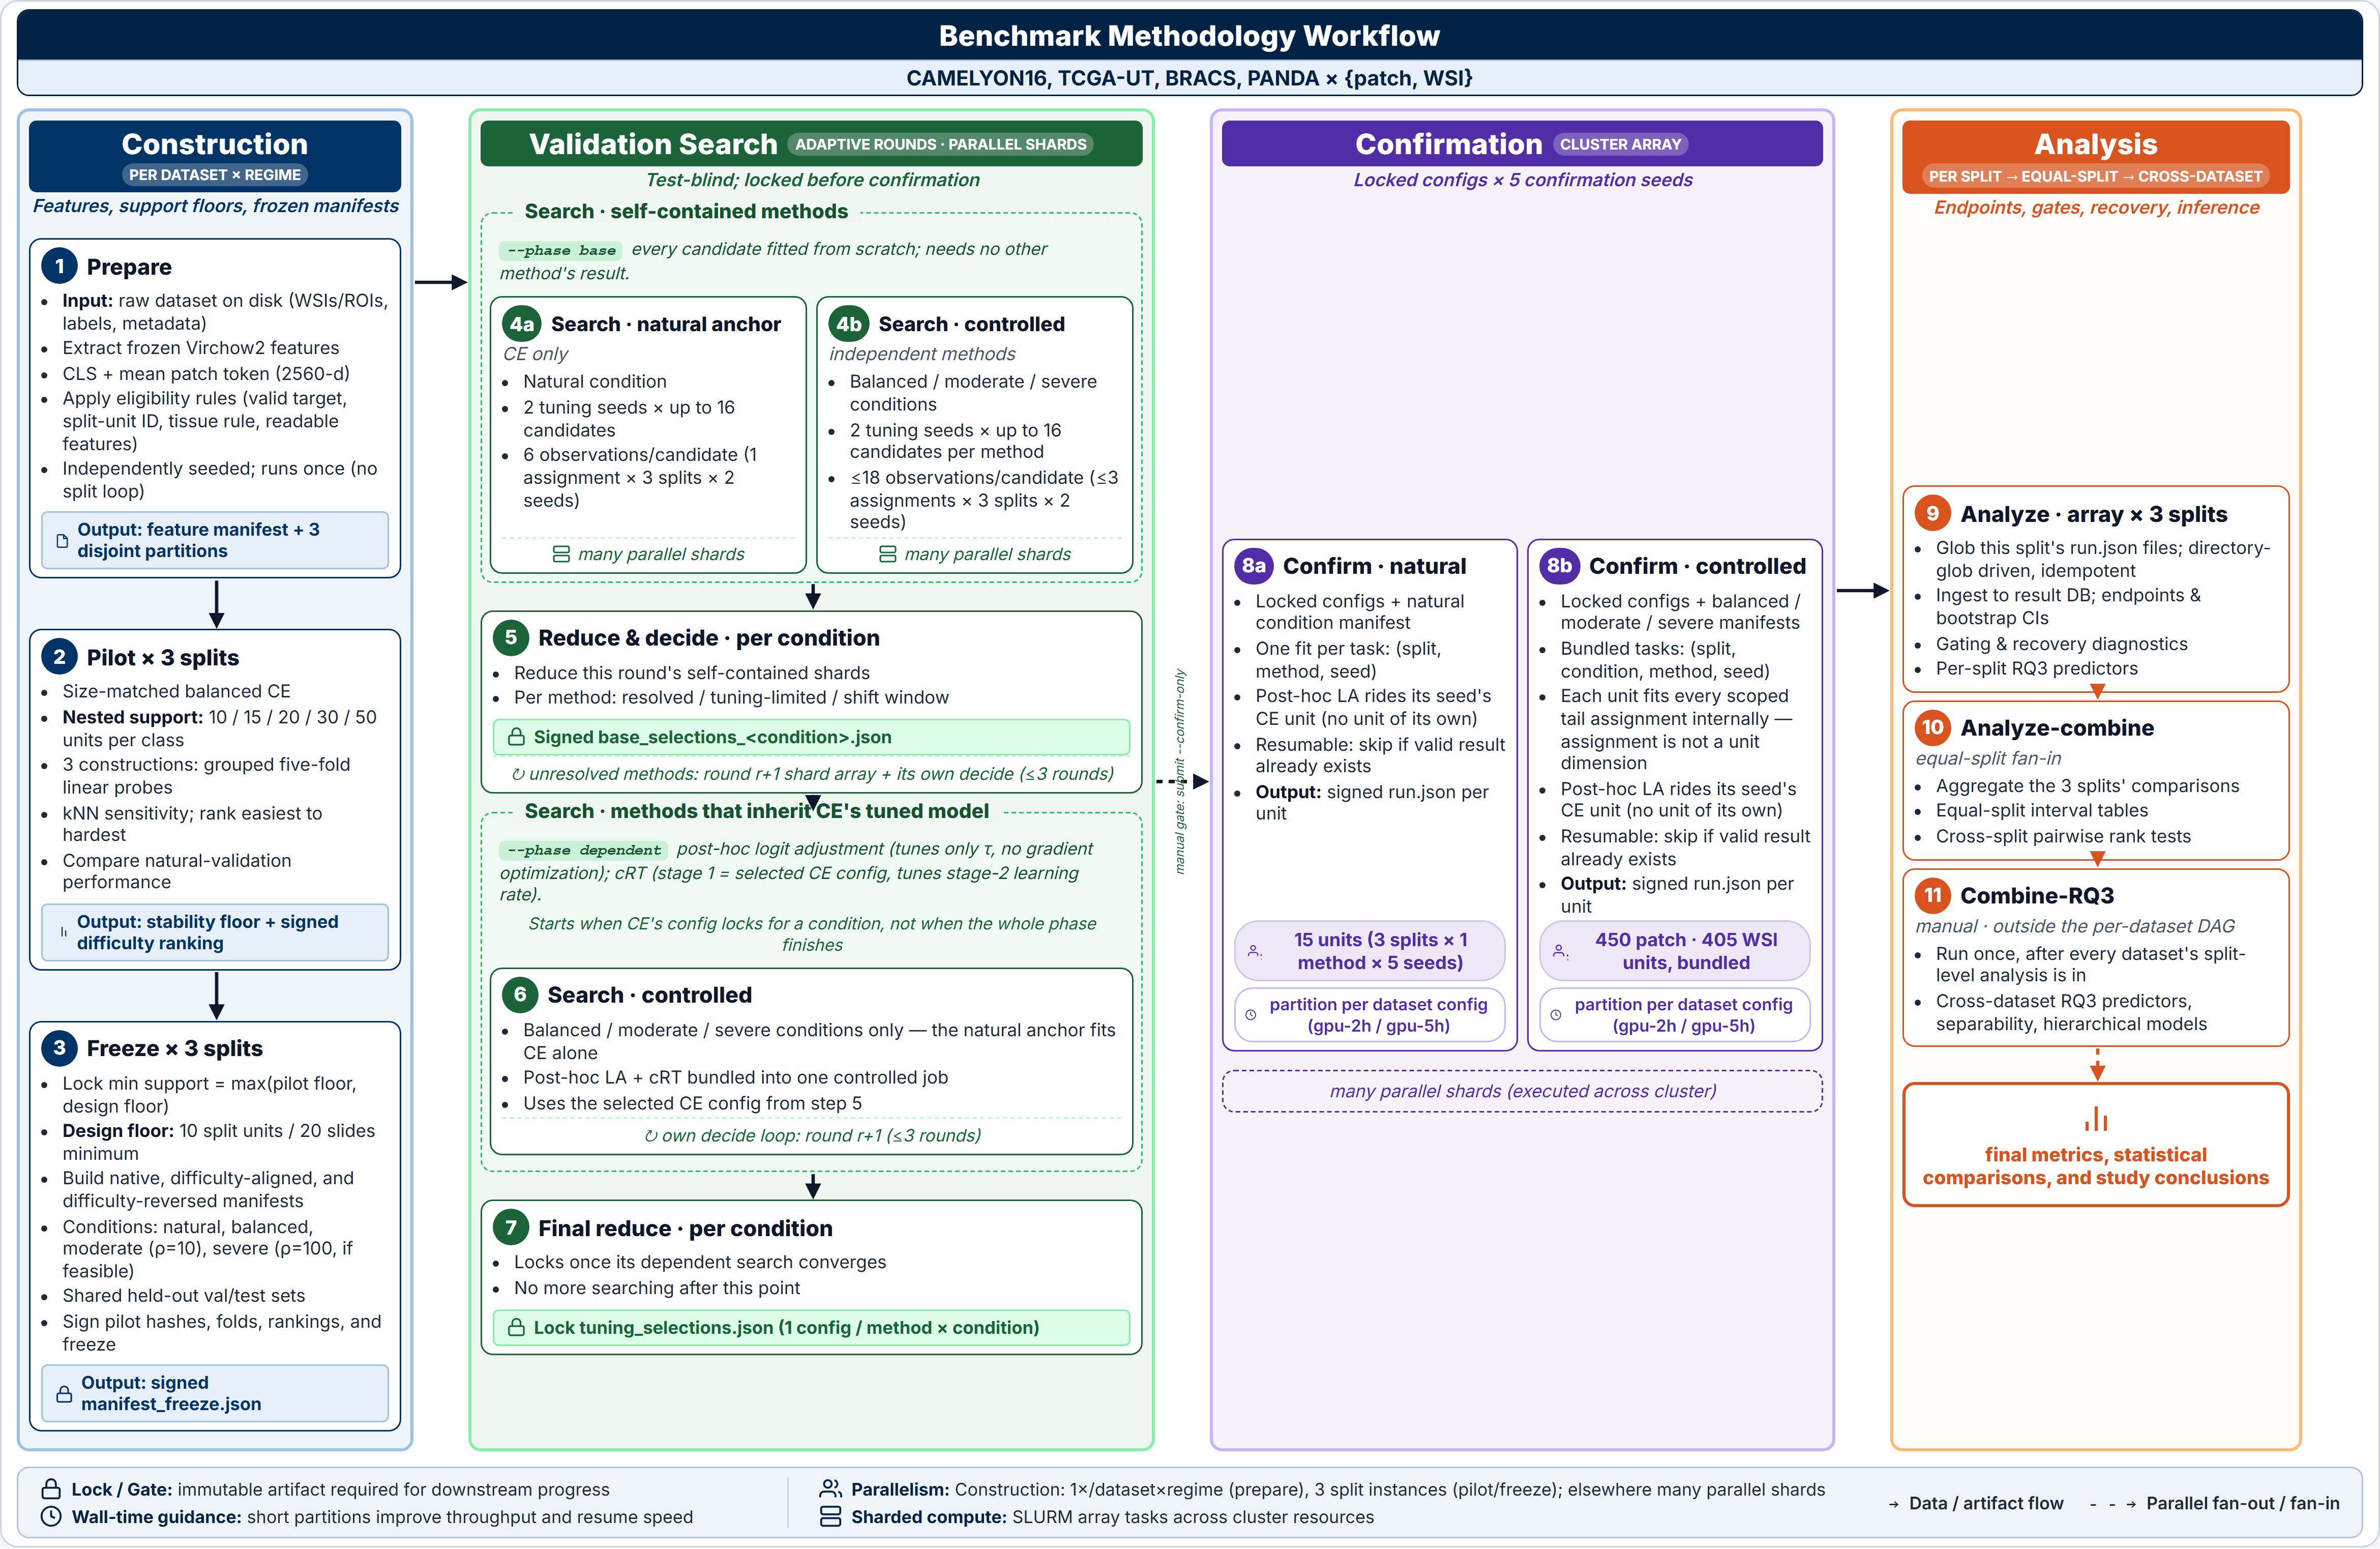
\includegraphics[width=0.92\linewidth,keepaspectratio]{assets/benchmark_patch.png}
  \caption{Operational workflow of the controlled class-imbalance benchmark.}
  \label{fig:benchmark-overview}
\end{figure}
\end{landscape}

This separation makes confirmation runs comparable without pretending that equal optimizer updates imply equal data exposure. With models fixed, evaluation can ask which endpoint was damaged and how much of that damage was recovered.

\subsection{Discrimination endpoints and aggregation units}
The primary endpoint is balanced accuracy, equal to macro recall for single-label multiclass prediction. Secondary discrimination outcomes are macro F1; per-class recall and F1; and head, body, and tail recall under the locked assignment. Classes are ranked by allocated training support: the first $\lceil K/3\rceil$ ranks are head, the last $\lceil K/3\rceil$ are tail, and intervening ranks are body; binary tasks have one head and one tail and no body. Ties follow the locked class ordering. Overall accuracy is descriptive. Patch predictions are summarized in two ways: patch-micro estimates treat eligible patches as predictions while uncertainty remains split-unit-clustered, and case-macro estimates first aggregate the metric contribution within each split unit so that heavily tiled cases do not dominate.

\subsection{Probability quality}
PANDA's patch target is binary (cancer versus benign), not the biopsy's ordinal ISUP grade; that grade is a slide-level label outside the patch prediction unit used here (Table~\ref{tab:datasets}), so no ordinal endpoint is reported. A patch-classification route to biopsy-level ordinal grading would require a new aggregation rule from patch-level cancer probability to a grade estimate, which the benchmark does not define; it is left to future work.

Probability-quality metrics ask whether the complete predicted distribution is useful, not only whether its largest entry names the correct class. Tail-group macro negative log likelihood (NLL) is the co-primary calibration endpoint because it gives each tail class equal weight and penalizes confident errors. Natural-prevalence NLL, macro NLL, multiclass Brier score, expected calibration error (ECE), and reliability diagrams provide secondary views. ECE uses 10 fixed equal-width bins and remains secondary because small classwise samples make bin estimates unstable.

Discrimination uses balanced-decision logits, whereas calibration uses target-prior-corrected probabilities before temperature scaling. Temperature-scaled outputs are secondary and never enter a recovery gate. Appendix~\ref{app:endpoints} defines every probability-quality equation, clipping at $10^{-12}$, score variants, and fixed-bin ECE.

\subsection{From imbalance deficit to mitigation recovery}
\label{sec:recovery}
Recovery is meaningful only when imbalance has first caused a measurable loss. The analysis therefore proceeds in two stages: compare size-matched balanced and imbalanced CE, then evaluate mitigation only on an endpoint that shows sufficiently large and statistically supported harm. One \emph{comparison unit} is a fixed dataset, imbalance severity, and tail assignment. A \emph{gate} is the prespecified eligibility rule that routes such a unit to the relevant recovery analysis; it is not a learned model component.

For a higher-is-better metric $M$, define the imbalance-induced deficit and recovery fraction at each imbalanced condition as
\begin{equation}
  \begin{aligned}
    D_M &= M(\text{balanced CE})-M(\text{imbalanced CE}),\\
    R_M &= \frac{M(\text{method on imbalanced data})
      -M(\text{imbalanced CE})}{D_M}.
  \end{aligned}
  \label{eq:recovery}
\end{equation}
$R_M=0$ denotes no recovery, $R_M=1$ recovery to the size-matched balanced CE reference, $R_M<0$ further deterioration, and $R_M>1$ performance beyond that reference. Because the balanced reference draws more unique tail independent units than any imbalanced condition at the same $T$, methods that only reweight or recalibrate the imbalanced training set cannot restore tail evidence that was never sampled; for that family $R_M<1$ may reflect an information ceiling rather than method failure, whereas resampling and synthesis methods are the only family for which $R_M=1$ is mechanically attainable. The full natural condition is descriptive and never enters $D_M$ or $R_M$: it has no size-matched balanced counterpart, so neither a deficit nor a recovery fraction is defined there. Fitting mitigation methods on it would therefore yield differences confounded by training volume as well as allocation, and the anchor is restricted to its CE reference for that reason.

\begin{figure}[H]
  \centering
  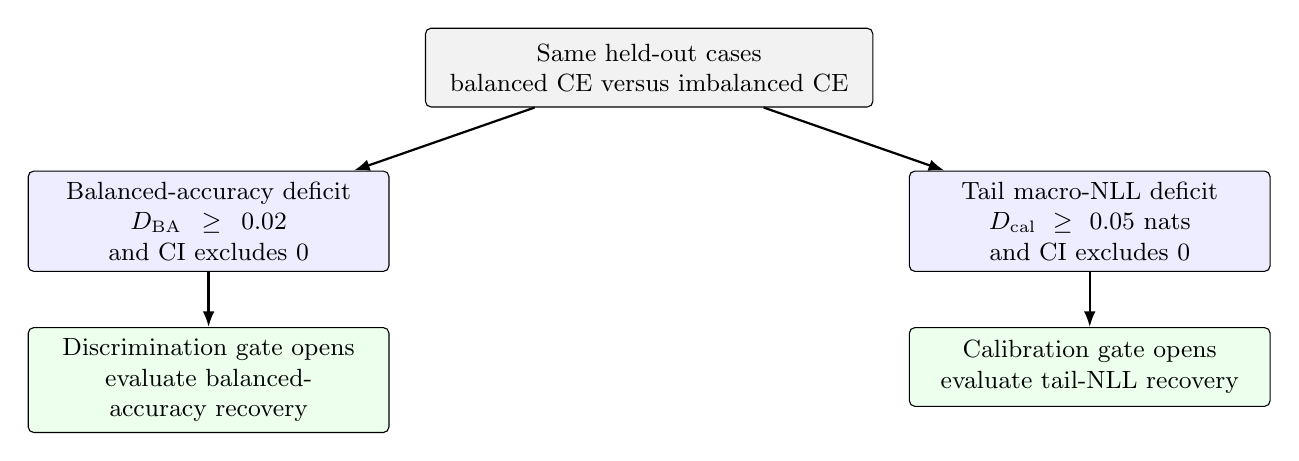
\begin{tikzpicture}[
    box/.style={draw, rounded corners=2pt, align=center, inner sep=4pt, font=\small, text width=4.3cm, minimum height=1.0cm},
    start/.style={box, fill=gray!10, text width=5.4cm},
    route/.style={box, fill=blue!7},
    result/.style={box, fill=green!7},
    arrow/.style={-{Latex[length=2mm]}, thick}
  ]
    \node[start] (contrast) {Same held-out cases\\balanced CE versus imbalanced CE};
    \node[route, below left=0.8cm and 0.45cm of contrast] (ba) {Balanced-accuracy deficit\\$D_{\mathrm{BA}}\geq0.02$ and CI excludes 0};
    \node[route, below right=0.8cm and 0.45cm of contrast] (cal) {Tail macro-NLL deficit\\$D_{\mathrm{cal}}\geq0.05$ nats and CI excludes 0};
    \node[result, below=0.7cm of ba] (barec) {Discrimination gate opens\\evaluate balanced-accuracy recovery};
    \node[result, below=0.7cm of cal] (calrec) {Calibration gate opens\\evaluate tail-NLL recovery};
    \draw[arrow] (contrast) -- (ba);
    \draw[arrow] (contrast) -- (cal);
    \draw[arrow] (ba) -- (barec);
    \draw[arrow] (cal) -- (calrec);
  \end{tikzpicture}
  \caption{Routing from an imbalance deficit to mitigation analysis. A comparison unit can enter through either gate or both. If neither rule is met, its CE deficits are still reported, but a recovery ratio is not interpreted. CI denotes the paired 95\% confidence interval.}
  \label{fig:gate-routing}
\end{figure}

Figure~\ref{fig:gate-routing} shows the two routes. The \emph{discrimination gate} opens when the CE balanced-accuracy deficit is at least \num{0.02} and its paired 95\% confidence interval excludes zero. The \emph{calibration gate} opens when the CE tail-group macro-NLL deficit, $\mathrm{NLL}_{\mathrm{tail}}(\mathrm{imbalanced\ CE})-\mathrm{NLL}_{\mathrm{tail}}(\mathrm{balanced\ CE})$, is at least \num{0.05} nats with a paired 95\% confidence interval excluding zero. Both rules are computed from CE runs on the same held-out cases before any mitigation method is compared. A comparison unit entering through the discrimination gate is evaluated for balanced-accuracy recovery; one entering through the calibration gate is evaluated for tail-calibration recovery; it may enter through both.

The two routes preserve an important distinction. Strong frozen features may leave balanced accuracy nearly intact while imbalance still biases tail probabilities, in which case a single discrimination rule would exclude methods designed to correct class priors. Conversely, the gates avoid unstable recovery ratios when no meaningful damage exists to recover. All CE deficits on both axes remain reported, including units that fail both rules. For the lower-is-better calibration axis, the sign-corrected deficit $D_{\mathrm{cal}}=\mathrm{NLL}_{\mathrm{tail}}(\mathrm{imbalanced\ CE})-\mathrm{NLL}_{\mathrm{tail}}(\mathrm{balanced\ CE})$ is the denominator and the method's tail-NLL improvement over imbalanced CE is the numerator, so Equation~\eqref{eq:recovery} retains the same interpretation. Recovery for other secondary metrics is descriptive and does not reopen a comparison unit that fails both gates.

\subsection{Uncertainty from independent units}
Uncertainty follows patients or cases rather than patches. A split-unit-clustered Bayesian bootstrap draws one positive Dirichlet weight per unit and carries that weight to all of its slides, patches, split appearances, and matched methods. Balanced CE, imbalanced CE, and mitigation runs receive the same unit weights and paired confirmation-seed draws; the complete deficit and recovery fraction are recomputed in every replicate.

A label-only preflight fixes \num{10000} resamples before predictions exist and checks class-cell representation, metric computability, paired weights, and weight variation. Kish effective counts and largest-weight shares identify cells dominated by too little independent evidence. Three split partitions are averaged with equal weight and are not treated as independent cohorts; five model initializations measure algorithmic variation, not five additional patient samples. Exact diagnostics, descriptive-only thresholds, and percentile-interval construction appear in Appendix~\ref{app:endpoints}.

\subsection{Paired testing and multiplicity control}
\label{sec:recovery-holm}
Confidence intervals and raw effect sizes are the main evidence. Hypothesis tests provide a supporting check for the prespecified primary methods. On the discrimination axis, the tested effect is the balanced-accuracy improvement over imbalanced CE. On the calibration axis, it is the reduction in tail-group macro NLL, oriented so that positive values indicate improvement. Recovery fractions are normalized effect summaries, not test statistics.

The raw two-sided $p$-value comes from a paired split-unit-block permutation test. This test represents the null hypothesis of no method difference by repeatedly swapping the method and imbalanced-CE labels within a split unit. The same swap is used for all of that unit's patches, split appearances, and matched confirmation seeds, preserving the paired design. All possible swaps are enumerated when feasible. Otherwise, \num{100000} random swaps are used with a plus-one correction; this gives a minimum attainable Monte Carlo $p$-value of approximately $10^{-5}$ and avoids reporting a simulated value of zero.

A \emph{test family} is the set of related hypotheses interpreted together. Testing many hypotheses increases the chance that at least one small $p$-value occurs by chance. Holm adjustment controls this family-wise error by ordering the raw $p$-values from smallest to largest, applying the strongest correction to the smallest value, and then proceeding stepwise with less stringent corrections. It provides this control without assuming that the tests are independent.

The confirmatory family holds one method per signal --- weighted CE (prevalence), class-balanced CE (nominal support), independent-support weighted CE (independent support), pilot-difficulty weighted CE (difficulty), and semantic-scale weighted CE (diversity) --- selected because all five share exactly one intervention level, a mean-one class weight on unmodified CE (Section~\ref{sec:five-family}), so a difference among them is attributable to the signal rather than to the mechanism. The family is specific to the patch regime and to the roster fitted here. Within one dataset, the family includes every gate-passing combination of primary method, gate, severity, and tail assignment; severities are not split into separate families. Holm adjustment is applied across the testable comparisons, while gated-out comparisons are recorded as not tested. Focal loss, train-time and post-hoc logit adjustment, balanced sampling, and every other roster member are exploratory: they retain the same effect estimates and confidence intervals but remain outside the confirmatory correction.

This is a revision of the family originally specified here, made before any recovery outcome was inspected: the prior family selected methods by intervention level (loss reweighting, prior correction, and resampling) with a rationale that assumed a second prediction regime the benchmark no longer carries. The revised, signal-based family is legitimate only because it was fixed before recovery outcomes were read, and only remains so if it is never revised again after that point.

\section{Explaining Heterogeneity}
\label{sec:rq3}
Why do some controlled comparisons show more damage or recovery than others? RQ1 and RQ2 estimate matched effects within a dataset and task. RQ3 then takes one step back and relates prespecified properties of each comparison to those effects. It neither predicts patient outcomes nor creates another method ranking. A \emph{controlled comparison} is one dataset, severity, and tail assignment cell for damage occurrence and magnitude; recovery comparisons additionally identify method and gate.

\paragraph{Outcomes to explain.}
The analysis is divided into three linked questions rather than one opaque combined model:
\begin{enumerate}
  \item \textbf{Damage occurrence:} did the comparison pass either prespecified deficit gate? Every controlled comparison contributes to this binary analysis.
  \item \textbf{Damage magnitude:} how large was the signed balanced-accuracy deficit? Every comparison contributes, including those with no damage or an apparent improvement under imbalance.
  \item \textbf{Mitigation headroom:} how much of the demonstrated deficit was recovered? Only gated comparisons contribute because recovery has no stable interpretation when there is no deficit to recover.
\end{enumerate}

\noindent These three outcomes correspond directly to the sequence introduced in RQ3: occurrence, magnitude, and conditional recovery.

\paragraph{Candidate explanations.}
Only quantities available without using test outcomes are eligible as predictors. Table~\ref{tab:rq3-predictors} separates the two primary predictors from the variables used only in sensitivity analyses.

\begin{table}[ht]
  \centering
  \footnotesize
  \begin{tabularx}{\linewidth}{@{}>{\raggedright\arraybackslash}p{0.23\linewidth}>{\raggedright\arraybackslash}p{0.49\linewidth}X@{}}
    \toprule
    Predictor & Question it represents & Model role \\
    \midrule
    Achieved imbalance ratio & How extreme was the realized head--tail allocation? & Primary, log-transformed \\
    Support--difficulty alignment $A=\operatorname{corr}(\log N_c,d_c)$ & Does greater allocated support go to more difficult classes ($A>0$), or does scarcity compound difficulty ($A<0$)? & Primary \\
    Intrinsic separability & How distinguishable are the classes in a common balanced frozen-feature reference, before condition-specific support is considered? & One-predictor sensitivity \\
    Condition-specific learnability & What remains learnable from the exact controlled training set? & One-predictor sensitivity \\
    Minimum independent support & How many distinct split units or slides support the scarcest class? & One-predictor sensitivity \\
    Effective patch support & How much patch support remains after accounting for within-case redundancy? & One-predictor sensitivity \\
    \bottomrule
  \end{tabularx}
  \caption{RQ3 predictors and their prespecified roles. Sensitivity predictors are fitted one at a time rather than added to the primary model.}
  \label{tab:rq3-predictors}
\end{table}

Intrinsic separability asks whether frozen Virchow2 features distinguish classes in a common balanced reference. Condition-specific learnability asks what remains learnable from the exact controlled training set. Both are measured on natural validation data without test outcomes. Minimum independent support and a patch-only redundancy-adjusted effective support are sensitivity predictors rather than replacements for patient or slide counts. Together these predictors measure the difficulty and independent-evidence dimensions of the signal taxonomy defined in the companion methods report \citep{queisler2026imbalanceMethods}, which the prespecified method roster itself covers only sparsely; RQ3 is therefore where those dimensions are examined directly rather than through a mitigation method.

One deliberately small model is fitted for each outcome. Every primary model contains only log achieved imbalance ratio and support--difficulty alignment, and each remaining predictor enters a separate one-predictor sensitivity model rather than being added to that primary model. Weak Gaussian priors and leave-one-group-out checks stabilize interpretation without claiming predictive generalization. Appendix~\ref{app:rq3} specifies probes, cross-fitting, ICC, effective support, model forms, MAP fitting, and sensitivity analyses.

RQ3 can therefore suggest which combinations of severity, difficulty, and support deserve follow-up, but it cannot turn the small set of dataset--target groups into general predictive evidence. The final section makes this and the benchmark's other interpretation limits explicit.

\section{Interpretation and Limitations}
\label{sec:limits}
The design supports deliberately narrow claims. Its strongest claim concerns effects of the training distribution under one frozen Virchow2 representation. It does not establish how end-to-end encoder fine-tuning would respond, whether another foundation representation would produce the same deficits, or whether constructed tails reproduce biological prevalence and referral pathways. The shared total $T$ isolates allocation by discarding some available examples; the full natural condition is therefore retained as a descriptive CE anchor, which places the controlled results on the scale of the complete training partition and of the dataset's own class prevalence. Because no mitigation method is fitted on that anchor, the benchmark reports no method comparison under natural prevalence, and its method claims are confined to the size-matched controlled conditions.

Method comparisons also identify methods, not universal mechanisms. Some interventions change sampling, objectives, or architecture together, and equal optimizer updates do not imply equal information exposure: post-hoc logit adjustment performs no gradient optimization, and cRT's second stage retrains only the classifier. Processed examples, unique exposures, accelerator time, memory, and model size are reported rather than treated as equal.

Independent support limits inference more strongly than raw patch count. BRACS patch classification is descriptive because its patch-micro Kish effective support remains below the prespecified threshold under patient-level bootstrap weights. This exclusion exposes an evidence limit rather than hiding an inconvenient result.

Finally, calibration is conditional on the natural held-out prevalence and cannot be transported to another deployment population without explicit prior-shift analysis. Within these boundaries, RQ1 estimates damage caused by controlled training allocation, RQ2 estimates recovery only where that damage is established, and RQ3 remains a hypothesis-generating explanation of between-comparison variation.

\clearpage
\appendix
\phantomsection
\addcontentsline{toc}{part}{Appendices}
\addtocontents{toc}{\protect\setcounter{tocdepth}{1}}
\section{Construction and Support Specification}
\label{app:construction}
This appendix records dataset eligibility, hierarchical sampling, support floors, allocation, and seed rules. These details implement the controlled contrast introduced in Section~\ref{sec:construction}; they do not add further estimands.

\subsection{Eligibility and representation}
Before examples are selected, each split unit is assigned to exactly one training, validation, or test partition, and all slides from that unit follow its assignment. A sample is excluded if it lacks a valid target or split-unit identifier, yields no patch under the dataset-specific tissue rule, lacks an annotation required for its patch label, or lacks readable frozen features. The same eligibility rules are applied before every imbalance condition.

TCGA-UT further excludes one of its 32 annotated cancer types, Diffuse Large B-cell Lymphoma, from the eligible target set. In every locked split this class contributes 20 participants and 20 slides, one slide per participant, so the 10\% split-unit and 5\% slide patch contribution caps (Section~\ref{app:construction-support}) admit essentially no count above the definitive floor: the class's set of cap-feasible patch counts covers only a few percent of the range between that floor and its native support, with the first infeasible count one unit above the floor. No shared total is therefore both tolerance-feasible and cap-feasible for this class, independent of severity or tail assignment. The remaining 31 cancer types are eligible and satisfy the tolerance search below.

All eligible patches enter the pool before condition-specific subsampling. The common classifier is a two-layer MLP with a 512-unit hidden representation, ReLU activation, dropout, and a linear class output. CFAL replaces the linear output with a prototype-based affinity head; OKO adds a training-only auxiliary head discarded at evaluation. Dataset provenance and complete preprocessing definitions remain in the companion dataset report \citep{queisler2026datasets}.

\subsection{Independent evidence and support floors}
\label{app:construction-support}
The independent-support rule of Section~\ref{sec:construction} is realized as a fixed per-class split-unit pool and, within it, a fixed slide pool, made available to the balanced and all imbalanced conditions: every condition draws its patches only from this pool. Table~\ref{tab:support-rules} states the selection order and caps.

\begin{table}[ht]
  \centering
  \footnotesize
  \begin{tabularx}{\linewidth}{@{}>{\raggedright\arraybackslash}p{0.30\linewidth}>{\raggedright\arraybackslash}p{0.24\linewidth}X@{}}
    \toprule
    Selection order & Contribution caps & What imbalance changes \\
    \midrule
    Split units, then slides within units, then patches; deterministic round-robin before any unit is revisited & $\leq10\%$ of a class's patch allocation per split unit; $\leq5\%$ per slide & Patches per class; the available split-unit and slide pools are unchanged \\
    \bottomrule
  \end{tabularx}
  \caption{Hierarchical selection and contribution caps. Every sample list reports per-class split-unit, slide, and patch counts, maximum contributions, and the fraction of the eligible independent pool retained.}
  \label{tab:support-rules}
\end{table}

\noindent The condition with the largest patch allocation for a class covers the fixed pool in full, so no unit in it goes unused by every condition together. A smaller condition for the same class, in particular a severe tail count well below that maximum, may leave some pool units untouched; this is the intended shape of an imbalanced allocation, not a violation of the shared pool.

The smallest defensible tail support is estimated before the definitive comparison with a \emph{support pilot}. These balanced CE runs ask when additional independent training units cease to materially improve natural-validation performance; they do not tune a hyperparameter or contribute observations to the definitive analysis. One pilot unit is a split unit, or a slide where split unit and slide coincide. Each selected unit contributes the same fixed quota $q_{\mathrm{patch}}$ of patches, distributed as evenly as possible over its eligible slides. The quota is the largest value the patient and slide contribution caps admit at every candidate level and every construction ordering, held fixed so increasing a pilot level adds independent units rather than patches per unit. A caps-admissible quota is necessary but not sufficient: a unit cannot supply more patches than it holds, so a unit is eligible for a candidate level only if its own inventory meets the candidate quota, and the quota at a given level is set from that level's order statistic of per-unit inventory over the eligible units rather than from the scarcest unit in one seeded ordering. A candidate level that no quota can satisfy is dropped from the curve rather than reusing a looser quota from a larger level.

Nested pilots compare $10,15,20,30,$ and $50$ units per class, or all available units when the scarcest class has fewer. They are repeated for three independently seeded \emph{construction orderings}. An ordering is a fixed sequence of eligible units; its prefix of length $m$ is simply the first $m$ units in that sequence. Thus the 15-unit pilot retains the same first 10 units as the 10-unit pilot and adds the next five. At lower levels of the hierarchy, every split unit has a fixed slide order and every slide has a fixed patch order. Figure~\ref{fig:construction-hierarchy} illustrates this nesting.

\begin{figure}[ht]
  \centering
  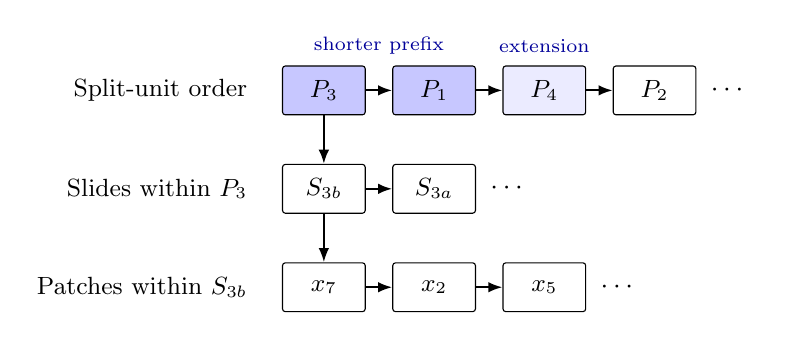
\begin{tikzpicture}[
    unit/.style={draw, rounded corners=1pt, minimum width=1.05cm, minimum height=0.62cm, font=\small},
    hierarchy/.style={font=\small, anchor=east},
    arrow/.style={-{Latex[length=1.8mm]}, thick}
  ]
    \node[hierarchy] at (-0.55,1.25) {Split-unit order};
    \node[unit, fill=blue!22] (p3) at (0.3,1.25) {$P_3$};
    \node[unit, fill=blue!22] (p1) at (1.7,1.25) {$P_1$};
    \node[unit, fill=blue!8] (p4) at (3.1,1.25) {$P_4$};
    \node[unit] (p2) at (4.5,1.25) {$P_2$};
    \node at (5.45,1.25) {$\cdots$};
    \draw[arrow] (p3) -- (p1);
    \draw[arrow] (p1) -- (p4);
    \draw[arrow] (p4) -- (p2);
    \node[font=\scriptsize, blue!60!black] at (1.0,1.82) {shorter prefix};
    \node[font=\scriptsize, blue!60!black] at (3.1,1.82) {extension};

    \node[hierarchy] at (-0.55,0) {Slides within $P_3$};
    \node[unit] (s3b) at (0.3,0) {$S_{3b}$};
    \node[unit] (s3a) at (1.7,0) {$S_{3a}$};
    \node at (2.65,0) {$\cdots$};
    \draw[arrow] (s3b) -- (s3a);
    \draw[arrow] (p3.south) -- (s3b.north);

    \node[hierarchy] at (-0.55,-1.25) {Patches within $S_{3b}$};
    \node[unit] (x7) at (0.3,-1.25) {$x_7$};
    \node[unit] (x2) at (1.7,-1.25) {$x_2$};
    \node[unit] (x5) at (3.1,-1.25) {$x_5$};
    \node at (4.05,-1.25) {$\cdots$};
    \draw[arrow] (x7) -- (x2);
    \draw[arrow] (x2) -- (x5);
    \draw[arrow] (s3b.south) -- (x7.north);
  \end{tikzpicture}
  \caption{Hierarchy behind one construction ordering. A seed fixes the split-unit sequence and the local slide and patch sequences. The darker unit boxes form a shorter prefix; the lighter third box is added, without replacing earlier units, when the prefix is extended.}
  \label{fig:construction-hierarchy}
\end{figure}

\noindent Because every larger pilot level extends the preceding prefix, adjacent levels are paired within an ordering and evaluated on the same natural-validation cohort. The smallest level whose next increment changes mean balanced accuracy by less than \num{0.01} and every class recall by less than \num{0.02} in all three orderings is the \emph{stability floor}; if none qualifies, the largest candidate is used.\footnote{No pilot level is exempt from the caps. A level is dropped from the curve when no quota satisfies both caps for every construction seed---e.g., the \num{5}\% slide cap needs at least 20 contributing slides, so a class whose split units mostly contribute a single slide can leave levels below 20 infeasible. Dropped levels are recorded in the frozen pilot report.}

The definitive minimum is the larger of this empirical stability floor and a prespecified design floor. Each class must contain at least 10 split units and 20 slides, or 20 slides when split unit and slide coincide, and any class-aware batch or set must contain at least two distinct same-class units. The 10-unit and 20-slide values are not estimated performance thresholds: they are the smallest counts compatible with the 10\% split-unit and 5\% slide contribution caps, respectively. A requested severity is reduced to the largest allocation satisfying both floors; a dataset is excluded if even its balanced condition fails them. Pilot quotas, curves, seeds, and resulting floors are frozen and reported with the definitive training sets.

Within these floors, one shared total $T$ is fixed for the balanced, moderate, and severe conditions of a split. Construction scores every integer total between the independent-support floor and the largest total any locked tail assignment's head class can support at $\rho_{\mathrm{target}}=100$, keeping only totals whose balanced allocation and whose every locked assignment's moderate and severe allocation satisfy the patch or slide contribution caps. Among these cap-feasible totals, the \emph{tolerance-feasible} set is those whose achieved moderate ratio falls in $[9,11]$ and whose achieved severe ratio falls in $[90,110]$ simultaneously, for every locked assignment. The largest tolerance-feasible total is checked against the true fixed-pool construction --- the same sampling procedure the definitive training sets use --- starting from the largest candidate and moving to the next largest until one is confirmed; that confirmed total is $T$. A dataset--regime with no tolerance-feasible total retains its largest independent-support- and cap-feasible total instead, subject to the infeasibility fallback and degeneracy rule below.

Before assigning support ranks, the largest balanced pilot level is used to measure class difficulty. Each of the three pilot constructions supplies one hierarchically matched draw in the sense of the companion methods report \citep{queisler2026imbalanceMethods}: every class contributes the same number of split units and every selected unit the same number of patches, so the probe sees equal independent support in every class rather than only equal patch counts. On each draw a class-balanced linear probe makes five-fold out-of-fold predictions with case/patient-disjoint \texttt{StratifiedGroupKFold} partitions. Class difficulty is $d_c=1-\overline{\mathrm{recall}}_c$, where recall is averaged across the three matched draws; five-neighbour kNN recall and the unmatched, patch-balanced-only probe error are retained as sensitivity evidence, the latter because a class ordering that changes between the matched and unmatched scores marks a class whose apparent difficulty is partly scarcity. Pilot hashes, folds, classwise scores, and the easiest-to-hardest ranking are signed. Equal scores retain native class order.

\subsection{Severity profiles and tail assignments}
A binary task needs only a head and a tail count, but a multiclass task also needs a rule for the classes between those extremes. The exponential construction places the $K$ class supports at equal intervals on a logarithmic scale. For a locked order from head ($i=0$) to tail ($i=K-1$), it assigns weights
\begin{equation}
  w_i(\rho_{\mathrm{target}})=\rho_{\mathrm{target}}^{-i/(K-1)},\qquad
  n_i^*=T\frac{w_i(\rho_{\mathrm{target}})}{\sum_{j=0}^{K-1}w_j(\rho_{\mathrm{target}})},
  \quad i=0,\ldots,K-1.
  \label{eq:construction}
\end{equation}
\noindent so the head-to-tail ratio is exactly $\rho_{\mathrm{target}}$ before integer rounding. For example, with four classes and $\rho_{\mathrm{target}}=100$, the unnormalized weights are approximately $1,0.215,0.046,$ and $0.01$; the two body classes lie geometrically between the head and tail instead of being assigned ad hoc counts. Binary targets use $n_{\mathrm{head}}^*/n_{\mathrm{tail}}^*=\rho_{\mathrm{target}}$ directly. The same exponential rule is applied to every multiclass dataset--regime, so a given $\rho_{\mathrm{target}}$ denotes the same allocation shape in each of them.

The values $n_i^*$ are real-valued targets, whereas a training set must contain whole patches or slides. \emph{Constrained integer allocation} converts them into usable class counts. Each target is rounded to the nearest integer and clipped to the class's support floor and available unique support. If the rounded counts do not sum to $T$, units are added to or removed from the classes with the largest rounding residuals until the total is exact. The resulting integers $n_i$ therefore satisfy $\sum_i n_i=T$ and every class-specific lower and upper bound while remaining close to the exponential targets under this deterministic adjustment.

Counts determine how many units a class contributes; construction orderings determine which units they are. One master ordering is created per class at each hierarchy level. Every condition selects a deterministic prefix, or a split-unit-round-robin extension of a prefix, from these same orderings: all fixed-pool split units and slides contribute before additional patches are allocated.

If a target ratio is infeasible, the same rule is applied to every dataset and regime: use the largest attainable ratio and report the requested ratio, achieved ratio, limiting class, realized counts, and binding support floor. Validation or test support is never reduced to manufacture feasibility. This general fallback is especially relevant to high-$K$ tasks, where an exponential profile must allocate support to many intermediate classes as well as the tail; it is not a dataset-specific exception. A stable lower-severity condition is preferred to a nominal $\rho=100$ condition supported by only a few independent units.

The fallback has a limit: a moderate or severe condition whose realized allocation is indistinguishable from the balanced condition---achieved ratio within a small tolerance of 1, or realized counts identical to the balanced training set---is not a lower-severity instance of the intended contrast but a null one, since the imbalance intervention did not occur. Such a condition is reported as degenerate rather than fitted and averaged with genuine moderate or severe conditions from other splits or assignments, and it is excluded from the imbalance deficit and recovery estimands in Section~\ref{sec:recovery}. Its requested ratio, achieved ratio, limiting class, and binding support floor are recorded alongside the exclusion, using the same fields every condition already reports.

The profile determines support by rank; the tail assignment maps semantic classes to those ranks. Native order is the clinical, ordinal, or natural-support order of the target; aligned and reversed order the classes by the difficulty scores $d_c$ measured above. Binary tasks retain native and reversed orientations only. A difficulty mapping that duplicates an earlier mapping in any locked split is omitted across that dataset--regime with its reason recorded. These three assignments separate interpretable mechanisms but do not exhaust all possible class-support mappings. Figure~\ref{fig:tail-assignments} illustrates the design.

\begin{figure}[ht]
  \centering
  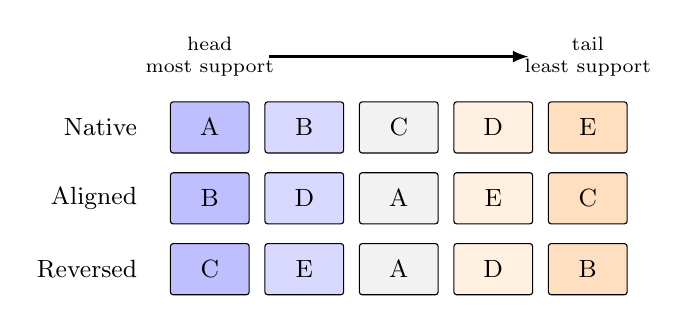
\begin{tikzpicture}[
    cls/.style={draw, rounded corners=1pt, minimum width=1.0cm, minimum height=0.65cm, font=\small},
    row/.style={font=\small, anchor=east},
    rank/.style={font=\scriptsize, align=center}
  ]
    \node[rank] at (0,1.55) {head\\most support};
    \node[rank] at (4.8,1.55) {tail\\least support};
    \draw[-{Latex[length=2mm]}, thick] (0.75,1.55) -- (4.05,1.55);

    \node[row] at (-0.8,0.65) {Native};
    \node[row] at (-0.8,-0.25) {Aligned};
    \node[row] at (-0.8,-1.15) {Reversed};

    \node[cls, fill=blue!25] at (0,0.65) {A};
    \node[cls, fill=blue!15] at (1.2,0.65) {B};
    \node[cls, fill=gray!10] at (2.4,0.65) {C};
    \node[cls, fill=orange!12] at (3.6,0.65) {D};
    \node[cls, fill=orange!25] at (4.8,0.65) {E};

    \node[cls, fill=blue!25] at (0,-0.25) {B};
    \node[cls, fill=blue!15] at (1.2,-0.25) {D};
    \node[cls, fill=gray!10] at (2.4,-0.25) {A};
    \node[cls, fill=orange!12] at (3.6,-0.25) {E};
    \node[cls, fill=orange!25] at (4.8,-0.25) {C};

    \node[cls, fill=blue!25] at (0,-1.15) {C};
    \node[cls, fill=blue!15] at (1.2,-1.15) {E};
    \node[cls, fill=gray!10] at (2.4,-1.15) {A};
    \node[cls, fill=orange!12] at (3.6,-1.15) {D};
    \node[cls, fill=orange!25] at (4.8,-1.15) {B};
  \end{tikzpicture}
  \caption{Illustrative tail assignments for a five-class target. Columns are support ranks fixed by the severity profile. Difficulty increases from B to C: aligned compounds difficulty with scarce support, while reversed compensates it.}
  \label{fig:tail-assignments}
\end{figure}

The random quantities are separated into five seed families so that changing one source of variation does not silently change another. Table~\ref{tab:seed-families} defines their roles.

\begin{table}[H]
  \centering
  \footnotesize
  \begin{tabularx}{\linewidth}{@{}l>{\raggedright\arraybackslash}p{0.37\linewidth}>{\raggedright\arraybackslash}X@{}}
    \toprule
    Seed family & Determines & Prespecified use \\
    \midrule
    Split-unit partition & Membership of the training, validation, and test cohorts & Three locked patient- or case-disjoint splits \\
    Tail assignment & Mapping of semantic classes to head--tail support ranks & Native, difficulty-aligned, and difficulty-reversed mappings from signed pilot evidence \\
    Construction & Split-unit, slide, and patch orderings and the selected evidence & Three pilot orderings and a disjoint fourth ordering for definitive training sets \\
    Initialization & Parameter initialization and optimization randomness & Two tuning seeds and five disjoint confirmation seeds \\
    Resampling & Bootstrap draws and permutation swaps & Uncertainty intervals and hypothesis tests only \\
    \bottomrule
  \end{tabularx}
  \caption{Seed families and their non-overlapping roles in the benchmark.}
  \label{tab:seed-families}
\end{table}

\noindent No seed is chosen based on test performance. The size-matched balanced training set and its trained CE baseline are shared by all tail assignments within a split.\footnote{At $\rho_{\mathrm{target}}=1$, every class receives equal support. Permuting semantic classes across support ranks therefore leaves the allocation unchanged, so tail assignment is not a meaningful factor for the balanced condition.} The same balanced predictions enter every assignment-specific deficit and are represented once in resampling data, avoiding duplicated balanced fits, bootstrap records, and artificial assignment variability.

\section{Endpoint and Inference Specification}
\label{app:endpoints}
This appendix defines secondary endpoints, score semantics, resampling, and diagnostics. Gates and recovery retain the main-text definitions in Section~\ref{sec:recovery}.

\subsection{Probability quality and calibration}
Let $N$ denote the number of held-out predictions in an aggregation unit, $C$ the number of classes, $y_i\in\{1,\ldots,C\}$ the true label, and $\hat{\mathbf{p}}_i\in[0,1]^C$ the predicted probability vector. Write $Y_i$ for the one-hot encoding of $y_i$.

Table~\ref{tab:score-variants} fixes which score variant enters each endpoint. For ordinary CE,
post-hoc logit adjustment, and train-time logit adjustment, the target-prior variant is the
correction defined in the companion methods report, using the natural-validation prior for the
corresponding test split. For every other method, the target-prior variant equals its raw logits.

\begin{table}[ht]
  \centering
  \small
  \begin{tabularx}{\linewidth}{@{}p{0.36\linewidth}X@{}}
    \toprule
    Endpoint or output & Score variant \\
    \midrule
    Balanced accuracy and all other discrimination endpoints
      & Balanced-decision logits: $z^{\mathrm{CE}}-\tau\log\widehat\pi$ for post-hoc logit adjustment; raw model logits for train-time logit adjustment and every other method. \\
    Tail-NLL deficit gate and tail-NLL recovery
      & Target-prior-corrected probabilities before temperature scaling. \\
    Reported NLL, Brier score, ECE, and reliability diagrams
      & Target-prior-corrected probabilities before temperature scaling; raw probabilities are retained as a separately labelled diagnostic. \\
    Temperature-scaled calibration outputs
      & Target-prior-corrected logits divided by one positive temperature fitted on natural-validation NLL and applied unchanged to test; these secondary outputs do not enter either recovery gate. \\
    \bottomrule
  \end{tabularx}
  \caption{Canonical mapping from evaluation endpoints to score variants.}
  \label{tab:score-variants}
\end{table}

\paragraph{Negative log likelihood.}
Natural-prevalence negative log likelihood (NLL), also called multiclass log loss, is
\begin{equation}
  \mathrm{NLL}=-\frac{1}{N}\sum_{i=1}^{N}\log \hat{p}_{i,y_i}.
  \label{eq:nll}
\end{equation}
\noindent Lower NLL indicates that more probability mass is assigned to the true class. The implementation clips $\hat{p}_{i,y_i}$ to $[10^{-12},1]$ before taking the logarithm. To prevent common classes from dominating probability-quality summaries, class-conditional NLL and macro NLL are
\begin{equation}
  \mathrm{NLL}_c=-\frac{1}{N_c}\sum_{i:y_i=c}\log \hat{p}_{ic},
  \qquad
  \mathrm{NLL}_{\mathrm{macro}}=\frac{1}{C}\sum_{c=1}^{C}\mathrm{NLL}_c,
  \label{eq:macro-nll}
\end{equation}
\noindent where $N_c$ is the number of held-out predictions from class $c$. Natural-prevalence NLL is the deployment-facing summary for the observed held-out cohort; macro NLL and unweighted head, body, and tail averages of $\mathrm{NLL}_c$ are tail-sensitive summaries.

\paragraph{Multiclass Brier score.}
The multiclass Brier score penalizes squared error across the full predicted distribution \citep{brier1950verification}:
\begin{equation}
  \mathrm{BS}=\frac{1}{N}\sum_{i=1}^{N}
  \left\|\hat{\mathbf{p}}_i-Y_i\right\|_2^2.
  \label{eq:brier}
\end{equation}
\noindent Lower values indicate better probability quality. The natural-prevalence score averages this error over the complete held-out cohort. Classwise scores apply the same full-distribution error only to predictions with $y_i=c$. Their unweighted averages provide head, body, and tail summaries.

\paragraph{Expected calibration error.}
For each prediction, let $\hat{y}_i=\arg\max_c\hat{p}_{ic}$ and $q_i=\max_c\hat{p}_{ic}$. Expected calibration error (ECE) partitions confidence into $B=10$ fixed equal-width bins on $[0,1]$ and compares mean confidence with empirical accuracy in each nonempty bin \citep{naeini2015obtaining}:
\begin{equation}
  \mathrm{ECE}=\sum_{b=1}^{B}\frac{|I_b|}{N}
  \left|\frac{1}{|I_b|}\sum_{i\in I_b}\mathbb{1}[\hat{y}_i=y_i]
  -\frac{1}{|I_b|}\sum_{i\in I_b}q_i\right|,
  \label{eq:ece}
\end{equation}
\noindent where $I_b$ contains the predictions assigned to bin $b$. ECE is secondary because it depends on binning and can be unstable with small classwise samples; its bootstrap uncertainty uses the same fixed bins and split-unit weights as the other endpoints. Reliability diagrams show the binwise confidence--accuracy relation overall and for the tail group.

Because checkpoints and hyperparameters are selected for natural-validation balanced accuracy, all probability-quality results describe discrimination-selected models rather than models optimized for calibration. The output semantics and prior-correction formulas of individual methods are defined in the companion methods report \citep{queisler2026imbalanceMethods}.

\subsection{Uncertainty from split-unit resampling}
The resampled split unit is the patient or participant where one is available, and the biopsy/WSI for PANDA and CAMELYON16. Each replicate reweights the observed split units rather than deterministically repeating each one exactly once, and the complete statistic is recomputed from those weights.

\paragraph{Label-only preflight.}
Before model training, \num{10000} bootstrap replicates are constructed using only split-unit identifiers, split membership, and class labels. \emph{Label-only} means that no predictions, performance values, or method identities are used; these replicates test whether the planned resampling scheme is valid before results can influence it. The count of \num{10000} is a prespecified Monte Carlo budget. It places about 250 replicates in each 2.5\% tail of a percentile interval, reducing simulation noise in the interval endpoints while remaining inexpensive at this label-only stage.

Each split unit draws an independent, continuous bootstrap weight in every replicate: a Bayesian bootstrap \citep{rubin1981bayesian} in which the $n$ observed units' weights are $n$ times a draw from a symmetric $\mathrm{Dirichlet}(1,\ldots,1)$ distribution over the $n$-simplex. This draw is almost surely strictly positive in every coordinate, so every unit contributes to every replicate; no split--class cell, including one contributed by a unit whose observed split-by-class pattern is unique among the cohort, can be emptied by an unlucky draw. A unit's observed contribution pattern---how many examples it supplies to each class in each test-split appearance---is still recorded and grouped into strata, but only to report per-stratum diagnostics; it no longer constrains the weight draw itself. A selected unit's weight is applied to all of its slides and patches in every split. Figure~\ref{fig:bootstrap-workflow} summarizes the workflow.

\begin{figure}[ht]
  \centering
  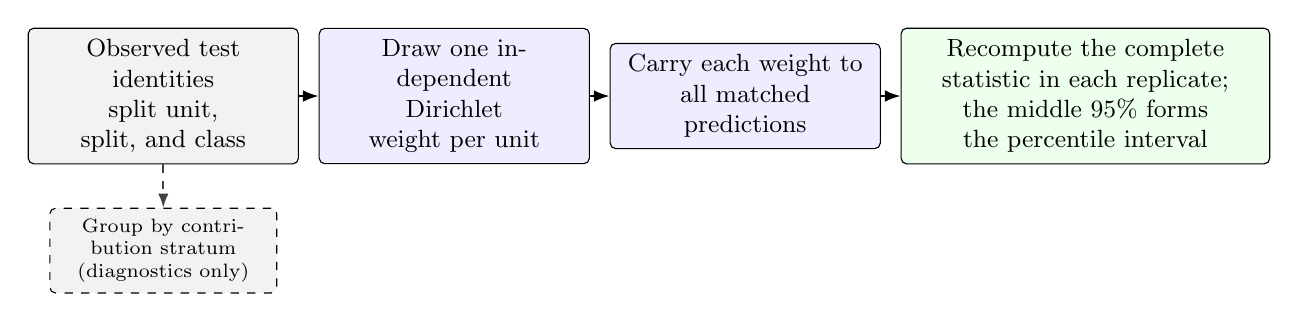
\begin{tikzpicture}[
    box/.style={draw, rounded corners=2pt, align=center, inner sep=4pt, font=\small, text width=3.15cm, minimum height=1.0cm},
    fixed/.style={box, fill=gray!10},
    sampled/.style={box, fill=blue!7},
    result/.style={box, fill=green!7, text width=4.4cm},
    note/.style={box, fill=gray!10, text width=2.6cm, font=\scriptsize, dashed},
    arrow/.style={-{Latex[length=2mm]}, thick},
    sidearrow/.style={-{Latex[length=1.8mm]}, thick, dashed, gray!50!black}
  ]
    \node[fixed] (identity) {Observed test identities\\split unit, split, and class};
    \node[sampled, right=0.25cm of identity] (draw) {Draw one independent\\Dirichlet weight per unit};
    \node[sampled, right=0.25cm of draw] (weights) {Carry each weight to\\all matched predictions};
    \node[result, right=0.25cm of weights] (interval) {Recompute the complete statistic in each replicate; the middle 95\% forms the percentile interval};
    \node[note, below=0.55cm of identity] (strata) {Group by contribution stratum\\(diagnostics only)};
    \draw[arrow] (identity) -- (draw);
    \draw[arrow] (draw) -- (weights);
    \draw[arrow] (weights) -- (interval);
    \draw[sidearrow] (identity) -- (strata);
  \end{tikzpicture}
  \caption{Split-unit-clustered Bayesian bootstrap workflow. The label-only preflight executes the identity, weight-draw, and stratum-diagnostic steps before predictions exist. After model fitting, the same paired per-unit weights are applied to every matched run.}
  \label{fig:bootstrap-workflow}
\end{figure}

\noindent The preflight verifies that every original split--class cell remains represented, every split-level metric is computable, one split unit receives the same weight across all of its split appearances, and every unit's resampled weight actually varies across replicates. Failure of any check stops the analysis rather than causing a replicate to be silently discarded.

The independent per-unit weight draw can still produce a replicate dominated by a few heavily weighted units. If split unit $i$ has class-specific bootstrap weight $v_i$, the \emph{Kish effective split-unit count}
\begin{equation}
  n_{\mathrm{Kish}}=\frac{\left(\sum_i v_i\right)^2}{\sum_i v_i^2}.
  \label{eq:kish}
\end{equation}
\noindent translates unequal case weights into the equivalent number of equally weighted split units. It decreases as weight concentrates. The preflight also records each split/class cell's number of contributing units and its largest unit-weight share. Table~\ref{tab:preflight} lists the three concentration checks; failing any one designates inference for that dataset--regime descriptive before training.

\begin{table}[ht]
  \centering
  \footnotesize
  \begin{tabularx}{\linewidth}{@{}>{\raggedright\arraybackslash}p{0.34\linewidth}X@{}}
    \toprule
    Diagnostic & Threshold for descriptive-only designation \\
    \midrule
    Effective split-unit count & 2.5th percentile of $n_{\mathrm{Kish}}$ across replicates below five \\
    Single-unit dominance & One unit supplies more than 50\% of a class's weight in more than 5\% of replicates \\
    Cell support & A split/class cell has fewer than five contributing units \\
    \bottomrule
  \end{tabularx}
  \caption{Label-only preflight concentration checks. All three are evaluated before predictions exist; the designation is recorded rather than used to discard replicates.}
  \label{tab:preflight}
\end{table}

\noindent A percentile rather than the minimum is used because the minimum across replicates is an extreme order statistic: its value falls as the replicate count rises, so a floor placed on it would encode the resampling budget rather than the support the cell actually carries. The diagnostic report and resampling seed are frozen with the analysis plan.

\paragraph{Intervals after model fitting.}
The three split-unit partitions are fixed design repetitions and are averaged with equal weight; they are not treated as three independent cohorts. Tail assignments remain separate unless an assignment-averaged estimand is explicitly reported. Within each case-bootstrap replicate, the five matched confirmation-seed indices are also resampled as paired blocks and averaged before the splits are combined. This captures algorithmic variation without pretending that five model initializations create five additional case cohorts.

Balanced CE, imbalanced CE, and each mitigation method receive the same split-unit multiplicities and confirmation-seed draws. The complete deficit and recovery fraction, including numerator and denominator, is recomputed in each replicate. The reported 95\% percentile interval spans the 2.5th to 97.5th percentiles of the resulting distribution. Patches are never bootstrapped independently.

\section{RQ3 Model Specification}
\label{app:rq3}
This appendix fixes diagnostic feature construction and deliberately small association models used for RQ3. None of these quantities is allowed to use test outcomes as an input predictor.

\paragraph{Measuring separability and learnability.}
The two diagnostics differ only in their reference set: intrinsic separability uses one fixed balanced reference subset per dataset and split, whereas condition-specific learnability uses the exact balanced or imbalanced training set of the condition being explained. Both are evaluated on the unchanged natural-validation cohort. Balanced $k$-nearest-neighbour (kNN) macro recall labels each validation embedding from its closest reference embeddings and gives every class equal weight. A \emph{linear probe} is a class-balanced linear classifier fitted on the frozen reference embeddings; its macro recall is the primary separability or learnability summary. Per-class nearest-neighbour error is reported descriptively to show which classes overlap. None of these diagnostics uses test labels or CE test performance; probes operate directly on patch embeddings.

\paragraph{Sensitivity to correlated patches.}
Unique split-unit and slide counts remain the primary support measures. As a secondary sensitivity analysis, within-case redundancy is discounted through the effective support $N_{\mathrm{eff},c}$ defined in the companion methods report \citep{queisler2026imbalanceMethods}, whose intraclass correlation (ICC) is computed here over split-unit or slide clusters within a class.

Two choices complete that definition for this benchmark. The clustered score is a class margin: the fixed intrinsic linear probe's logit for class $c$ minus its largest competing logit. It is evaluated by \emph{cross-fitting}, so each observation is scored only by a probe trained without it, and the resulting ICC estimate is clipped to $[0,1]$. Effective support is a sensitivity measure and not a replacement for independent-unit counts, with patient count also examined when patients contribute multiple slides.

\paragraph{Three deliberately small association models.}
One model is fitted for each of the three RQ3 outcomes. The occurrence model handles the yes/no gate result; the magnitude and recovery models handle continuous outcomes. Every primary model contains exactly two predictors: the log achieved imbalance ratio and support--difficulty alignment $A$. The magnitude model also uses each deficit's bootstrap standard error so that a noisy estimated deficit is not treated as an exact observation.

Comparisons from the same dataset--target group can share a baseline level of difficulty. A \emph{random intercept} allows each group to have its own starting level while estimating common associations with imbalance and alignment. This adjustment is important because the analysis pools several severities and assignments from the same group. The recovery model omits method-specific effects because the small number of gated units cannot support them.

The remaining predictors in Table~\ref{tab:rq3-predictors} are fitted one at a time in separate sensitivity models. They are not combined with one another or with the two primary predictors because only a few independent dataset--target groups are available and the candidate predictors are strongly confounded. No interactions are fitted.

Parameters are estimated by maximum a posteriori (MAP) fitting: ordinary model fit is combined with weak zero-centered Gaussian priors that discourage extreme slopes and variance estimates in this small sample. A leave-one-dataset--target-group-out check then refits the magnitude model while withholding one complete group at a time. This is only a coarse stability check, not evidence of predictive generalization. Model definitions, predictor roles, and priors are frozen before recovery outcomes are inspected, and all RQ3 conclusions remain hypothesis-generating.

\section{Training, Tuning, and Execution Specification}
\label{app:training}
This appendix records exact update budgets, validation-search rules, replication, and resource accounting. Main-text interpretation depends only on their matched and test-blind use.

\subsection{Update budgets and checkpoint selection}
The frozen encoder, classifier family, optimizer family, batch definition, augmentation, and numerical precision are held fixed. Training is budgeted only in optimizer updates; epochs are neither a stopping rule nor a unit of comparison. With $B$ the locked batch size and $T$ the common controlled support, the reference budget is
\begin{equation}
  U=30\left\lceil\frac{T}{B}\right\rceil
  \label{eq:update-budget}
\end{equation}
\noindent updates, corresponding to 30 reference passes through $T$ examples under ordinary sampling. Table~\ref{tab:budgets} allocates that budget to the methods that do not consume it in a single stage.

\begin{table}[ht]
  \centering
  \footnotesize
  \begin{tabularx}{\linewidth}{@{}>{\raggedright\arraybackslash}p{0.26\linewidth}X@{}}
    \toprule
    Method & Optimizer updates \\
    \midrule
    Single-stage default & $U$; every method not listed below \\
    cRT & $U$ stage one, then $\lceil0.2U\rceil$ stage two on the classifier only \\
    Natural anchor (CE only) & Equation~\eqref{eq:update-budget} at its own support; descriptive, enters no matched contrast \\
    \bottomrule
  \end{tabularx}
  \caption{Allocation of the reference update budget $U$. Balanced sampling and replacement do not change $U$. Processed examples, unique-example exposures, and updates are all reported.}
  \label{tab:budgets}
\end{table}

\noindent Within a run, the reported checkpoint is fixed by three rules:
\begin{enumerate}
  \item Validation metrics are stored at fixed update intervals. The interval is scaled per dataset so the number of stored validation checkpoints is comparable across the widely differing controlled supports $T$, and the resolved value is recorded with every run.
  \item The selected checkpoint maximizes natural-validation balanced accuracy; macro F1 and then lower NLL are deterministic tie-breakers.
  \item Test predictions are produced once from that locked checkpoint.
\end{enumerate}

\subsection{Control grids and adaptive validation search}
\label{app:controls}
Hyperparameter comparisons are bounded by a common validation-search budget rather than by restricting every method to one tuned quantity, and the search adapts within a prespecified envelope rather than committing to a single fixed grid. Every trainable method draws its learning rate from the common envelope
\begin{equation}
  \eta\in\{\num{1e-5},\num{3e-5},\num{1e-4},\num{3e-4},\num{1e-3},\num{3e-3},\num{1e-2}\}.
  \label{eq:learning-rate-grid}
\end{equation}
\noindent Table~\ref{tab:controls} lists each method's imbalance-specific control. Focal loss, CE + soft F1, and CE + soft MCC draw their strength from a seven-value envelope searched through the same adaptive window as the learning rate; every other control is a fixed four-value grid, since its domain is naturally bounded. Both axes follow the search below, in which an edge winner is never accepted as an optimum: a bounded number of window shifts replaces a single fixed grid, at the cost of one new candidate per shift.

\begin{table}[ht]
  \centering
  \footnotesize
  \begin{tabularx}{\linewidth}{@{}lX@{}}
    \toprule
    Method or family & Candidate method-specific control \\
    \midrule
    Balanced sampling / weighted CE & strength $\in\{0.25,0.5,0.75,1\}$ \\
    Focal loss & $\gamma\in\{0,0.5,1,1.5,2,4,8\}$ envelope; active window starts at $\{0.5,1,1.5,2\}$ \\
    Logit adjustment & $\tau\in\{0.25,0.5,1,2\}$ \\
    CE + soft F1 / soft MCC & auxiliary weight $\in\{0,0.25,1,4,16,64\}$ envelope; active window starts at $\{0.25,1,4,16\}$ \\
    CFAL & affinity bandwidth $\sigma\in\{0.25,1,2,4\}$ \\
    OKO & odd-class count $k\in\{1,2,4,8\}$, capped by $K-1$ \\
    Class-balanced CE & $\beta\in\{0.9,0.99,0.999,0.9999\}$; saturation points $1/(1-\beta)\in\{10,100,1000,10000\}$, matched to $n_c$'s range \\
    Independent-support weighted CE & $\beta\in\{0.8,0.95,0.99,0.999\}$; saturation points $\{5,20,100,1000\}$, scaled down to $G_c$'s range, plus a matched-$\beta$ arm at class-balanced CE's tuned $\beta$ (Section~\ref{sec:five-family}) \\
    Pilot-difficulty weighted CE & $\tau\in\{0.25,0.5,0.75,1\}$ \\
    Semantic-scale weighted CE & $\tau\in\{0.25,0.5,0.75,1\}$; reweighting begins at reference pass 6 of 30 (Section~\ref{sec:five-family}) \\
    \bottomrule
  \end{tabularx}
  \caption{Prespecified method-specific controls, crossed with the active window of the learning-rate envelope in Equation~\eqref{eq:learning-rate-grid}. Focal loss and the two soft-label hybrids search their listed envelope through an adaptive four-value window; every other row is a fixed four-value grid. cRT has no imbalance-strength grid; only its stage-two learning rate is selected separately. The class-balanced and independent-support $\beta$ grids are matched saturation points on the effective-number transform, scaled to each method's own counting unit (Section~\ref{sec:independent-support}).}
  \label{tab:controls}
\end{table}

\begin{center}
  \fbox{%
  \begin{minipage}{0.94\linewidth}
    \small
    \textbf{Adaptive window search}, run once per method, dataset, and imbalance severity.
    \begin{enumerate}\setlength{\itemsep}{1pt}
      \item Initialize each active window to four adjacent envelope values: $\{\num{1e-4},\num{3e-4},\num{1e-3},\num{3e-3}\}$ for the learning rate, and the start listed in Table~\ref{tab:controls} for an adaptive strength axis.
      \item Fit the active learning-rate window crossed with the method's strength window or fixed grid: at most 16 candidates in any one round. Candidates fitted in an earlier round are reused, never retrained.
      \item If an axis's winning value is interior to its window, record the axis as \emph{resolved} and stop searching it.
      \item If the winner is an edge value and the envelope extends further in that direction, shift the window one position toward that edge and return to step 2. Only the single newly added candidate is fitted; the three overlapping candidates are reused.
      \item If the winner is an edge value at the envelope's boundary, retain the boundary value and record the axis as \emph{tuning-limited}.
    \end{enumerate}
    \textbf{Round bounds.} At most three rounds on the learning-rate axis, three on focal loss's $\gamma$ axis, and two on the soft-F1 and soft-MCC strength axis, each bounded by its envelope's length. A resolved or tuning-limited axis is never retrained in a later round.
  \end{minipage}}
\end{center}

For weighted CE, balanced sampling, focal loss, CE + soft F1, and CE + soft MCC, an imbalance-specific strength of zero is mathematically identical to plain CE at the same learning rate: it applies no class reweighting or sampling adjustment, reduces the focal term to the plain cross-entropy loss, or drops the auxiliary term entirely. That value is therefore excluded from the searched window, and its metrics are copied from CE's already-fitted same-learning-rate run rather than retrained, giving each of these five methods one additional comparison point at no extra training cost.

Four method families deviate from the search above. CE and methods without a meaningful imbalance-specific control search the learning-rate envelope alone. Train-time logit adjustment is tuned jointly over $\tau$ and learning rate, with $\tau$ held to its fixed grid. Post-hoc logit adjustment inherits the selected CE model and tunes only $\tau$, because it performs no gradient optimization. cRT inherits the selected CE configuration for stage one and selects its stage-two classifier learning rate separately from the common grid. Temperature scaling, when reported, fits one positive scalar on natural-validation NLL after model and checkpoint selection and applies it unchanged to test logits \citep{guo2017calibration}.

\subsection{Replication, locking, and records}
Selection and replication follow prespecified units rather than per-run judgement:
\begin{itemize}\setlength{\itemsep}{1pt}
  \item \textbf{Tuning seeds.} Every candidate is fitted with the same two tuning initialization seeds for each prespecified split-unit partition and tail assignment.
  \item \textbf{Selection unit.} One method, dataset, and imbalance severity. Within it, natural-validation balanced accuracy is averaged across both tuning seeds, all tuning splits, and all tail assignments; the highest aggregate is selected, with macro F1 and then lower NLL as deterministic tie-breakers.
  \item \textbf{Locking.} The chosen configuration is locked before any of the five disjoint confirmation initialization seeds is fitted and before test evaluation. Tuning runs never enter confirmation effect estimates.
  \item \textbf{Confirmation.} Each locked partition and tail assignment is repeated with the five confirmation seeds. Exactly three split-unit partition seeds are used; a dataset--regime unable to produce all three valid splits under the independent-support floors is excluded from the corresponding confirmatory analysis.
  \item \textbf{Matching.} The two runs of a controlled contrast (Appendix~\ref{app:terms}) share split-unit partition, tail assignment, confirmation-seed index, and held-out cases, so the contrast does not mix the intended change with a different cohort or replication.
  \item \textbf{Failures.} The unit of replication and all missing or failed runs are reported. A failed run is never silently replaced using a test-informed seed.
\end{itemize}

Split counts, support floors, condition training sets, tuning and confirmation seeds, method grids, and update budgets are frozen in the signed analysis plan before the first definitive fit. Every candidate fitted, every window shift, and the resolved-or-tuning-limited outcome of each axis are recorded there before the corresponding method enters confirmation. No test data and no confirmation-stage result ever informs a shift, and no grid is changed once confirmation training begins.

For every realized condition, the experiment record contains
\begin{itemize}\setlength{\itemsep}{1pt}
  \item dataset version and eligibility rules;
  \item split-unit, slide, and patch identifiers by partition;
  \item requested and achieved $T$ and $\rho$, and the class assignment;
  \item all seed families and their tuning, confirmation, pilot, or definitive roles;
  \item pilot patch quota and bootstrap-preflight diagnostics;
  \item model and optimizer configuration, candidate grid, and selected checkpoint;
  \item environment identifier and test-prediction hash.
\end{itemize}
\noindent Deviations are dated and justified before the affected test labels are accessed.

Computational cost is separated into validation search and locked-configuration fitting, and reported as wall-clock training time, accelerator-hours, and peak accelerator memory; total and trainable parameter counts; and effective passes through unique training examples. Costs include every method-specific stage, including both cRT stages, but exclude the one-time frozen-feature extraction shared by all methods. Hardware and software environments are recorded with each run.


\section{Terminology}
\label{app:terms}
\begin{description}
  \item[Natural anchor.] The full eligible natural training partition, fitted with the CE reference alone. It is descriptive and may have a different size from controlled conditions.
  \item[Size-matched balanced reference.] A training subset with total support $T$ and approximately equal class counts; it defines the counterfactual reference in $D_M$.
  \item[Imbalance severity.] The requested training allocation summarized by $\rho$; achieved severity is computed from realized integer counts.
  \item[Pilot level.] A candidate number of independent training units per class used in the balanced CE support-stability study.
  \item[Tail assignment.] The locked mapping from semantic classes to positions in the constructed support profile.
  \item[Comparison unit.] One dataset, imbalance severity, and tail assignment evaluated together.
  \item[Deficit gate.] A prespecified threshold rule that determines whether an observed discrimination or calibration deficit is large and precise enough for recovery analysis.
  \item[Imbalance deficit.] The paired balanced-CE minus imbalanced-CE difference at common $T$ and on the same held-out cases.
  \item[Recovery.] A method's improvement over imbalanced CE divided by the evidenced imbalance deficit.
  \item[Kish effective split-unit count.] The equally weighted split-unit count with the same weight concentration as one bootstrap replicate.
  \item[Intraclass correlation.] The estimated similarity of class margins from patches belonging to the same split-unit or slide cluster.
  \item[Patch-micro estimate.] A metric computed over eligible patch predictions, with split-unit-clustered uncertainty.
  \item[Case-macro estimate.] An equal-weight aggregation over slides or split units, limiting domination by heavily tiled cases.
  \item[Self-contained search.] The validation-search phase in which every candidate is fitted from scratch, needing no other method's result.
  \item[CE-inherited search.] The validation-search phase for post-hoc logit adjustment and cRT, which reuse a condition's selected CE configuration and tune only what remains open for that method ($\tau$ for post-hoc logit adjustment; the stage-two learning rate for cRT), and so cannot begin until that condition's CE search has resolved.
\end{description}

\clearpage
\bibliographystyle{plainnat}
\bibliography{references}

\end{document}
